\documentclass[12pt,fleqn,a4paper,oneside]{mybook} %Final!!!
%\documentclass[11pt,fleqn,a4paper,draft]{mybook} %DRAFT - highlights overflow, leaves out images

%\usepackage{microtype}
\usepackage[slovak]{babel}
\usepackage[utf8]{inputenc}
\usepackage[T1]{fontenc}
\usepackage[normalem]{ulem}
\usepackage{mathtools}  					
\usepackage{graphicx}
\usepackage{subfigure}
\usepackage{enumerate}
\usepackage{etoolbox}                       %Problematic URL in reference
\apptocmd{\sloppy}{\hbadness 10000\relax}{}{}%Removes badness warnings
%This is to remove warnings resulting by otherwise OK URL's
\usepackage[hyphens]{url}
\usepackage{notes}


%This custom command defines how the literal menus look like.
\newcommand{\gui}[1]{{\emph{#1}}} %Gui commands, icon names, buttons
 % All code, functions, variables are typed like this
\newcommand{\code}[1]{{\lstinline[columns=fixed]{#1}}}

\newcommand{\angl}[1]{{\footnote{\emph{angl.}\ {#1}}}} %Shorthand english equivalent


\usepackage[left=25mm,right=25mm,top=25mm,bottom=25mm,paperwidth=210mm,paperheight=297mm,includehead]{geometry}

\usepackage{titlesec}
\titleformat{\chapter}[hang]{\normalfont\huge\bfseries}{\thechapter}{1em}{}


\DeclarePairedDelimiter{\diagpars}{(}{)}
\newcommand{\diag}{\operatorname{diag}\diagpars}

\let\oldhat\hat
\renewcommand{\vec}[1]{\boldsymbol{\mathbf{#1}}}
%\renewcommand{\hat}[1]{\oldhat{\boldsymbol{\mathbf{#1}}}}


\usepackage{amsthm}
\usepackage{etoolbox}% http://ctan.org/pkg/etoolbo
\theoremstyle{definition}
\newtheorem{exmp}{Pr\'{i}klad}[chapter]
\AtEndEnvironment{exmp}{\null\hfill\qedsymbol}

\usepackage{listings,color} 			    %To list Matlab code
\definecolor{mygrey}{gray}{0.5}	        %Define a gray color
\lstset{
basicstyle=\ttfamily,
numbers=none,
commentstyle=\color{mygrey},
breaklines=true,
}
%extended Matlab language
\lstdefinelanguage{exMatlab}[]{Matlab}      %Defining expanded Matlab
{morekeywords={rng,pyulear,plot,hold,randn,filter,length,abs,periodogram,fft,sin,randn,xcorr,fminsearch,dlqr,predmodelqp,dlyap,ones,linprog,quadprog,optimset,qpOASES,qpOASES_sequence,sysStruct,probStruct,mpt_control,volume,hull,extreme,mpt_exportc,mpt_getInput,sdpvar,blkdiag,sdpsettings,solvesdp,geomean,double},
sensitive=true,
alsoletter={_}
}



\pagestyle{empty}

\begin{document}
%%%%%%% Zaciaatok %%%%%%%%
\renewcommand\thepage{\roman{page}}
\pagenumbering{roman}
\thispagestyle{empty}

\noindent \begin{center}
\textbf{{\large{}SLOVENSKÁ TECHNICKÁ UNIVERZITA V BRATISLAVE}}\\
\textbf{{\large{}STROJNÍCKA FAKULTA}}\textbf{\large{} }\\
\vspace{3cm}
\par\end{center}

\noindent \begin{center}
\vspace{3cm}
\par\end{center}



\begin{center}
\textbf{\textsc{\Large{}AeroShield: Miniatúrny experimentálny modul aerokyvadla}}\\
\par\end{center}{\Large \par}

\begin{center}
\textbf{\large{}Bakalárska práca}\\
\par\end{center}{\large \par}

\begin{center}
{\large{}SjF-číslo b. práce}\\
\par\end{center}{\large \par}



\vfill
\noindent \textbf{\large{}2022} \hfill \textbf{\large{}Bc. Peter Tibenský}
\cleardoublepage

\thispagestyle{empty}

\noindent \begin{center}
\textbf{{\large{}SLOVENSKÁ TECHNICKÁ UNIVERZITA V BRATISLAVE}}\\
\textbf{{\large{}STROJNÍCKA FAKULTA}}\textbf{\large{} }\\
\vspace{3cm}
\par\end{center}

\noindent \begin{center}
\vspace{3cm}
\par\end{center}



\begin{center}
\textbf{\textsc{\Large{}AeroShield: Miniatúrny experimentálny modul aerokyvadla}}\\
\par\end{center}{\Large \par}

\begin{center}
\textbf{\large{}Bakalárska práca}\\
\par\end{center}{\large \par}

\begin{center}
{\large{}SjF-12345-67890}\\
\end{center}


\vfill
\begin{flushleft}
$\begin{array}{ll}
\text{Študijný odbor:}&\text{Automatizácia a informatizácia strojov a procesov}\\
\text{Študijný program:}&\text{5.2.14 automatizácia}\\
\text{Školiace pracovisko:}&\text{Ústav automatizácie, merania a aplikovanej informatiky}\\
\text{Vedúci záverečnej práce:}&\text{Ing. Mgr. Anna Vargová.}\\
\text{Konzultant:}&\text{Ing. Erik Mikuláš}\\
\end{array}$
\end{flushleft}
\vspace{0.5cm}
\noindent \textbf{\large{}Bratislava, 2022} \hfill \textbf{\large{}Peter Tibenský}
\cleardoublepage

Úlohou študenta je navrhnúť, realizovať a sériovo vyrobiť rozširovací modul pre prototypizačnú platformu Arduino v rámci open-source projektu „AutomationShield“. Jedná sa o návrh miniaturizovaného laboratórneho experimentu so spätnoväzobným riadením tzv. aerokyvadla, spolu s ovládacím softvérom a inštruktážnymi príkladmi. Študent navrhne plošný spoj v CAD prostredí DipTrace, vytvorí programátorské rozhranie (API) v jazyku C/C++ pre Arduino IDE, ďalej pre MATLAB a Simulink. Študent manažuje verzie projektu v Git pre GitHub a píše úplnú dokumentáciu v MarkDown.

\cleardoublepage

	

\null
\vfill
\noindent
\section*{Čestné prehlásenie}

Vyhlasujem, že predloženú záverečnú prácu som vypracoval samostatne pod vedením vedúceho záverečnej práce, s použitím odbornej literatúry a ďalších informačných zdrojov, ktoré sú citované v práci a uvedené v zozname použitej literatúry. Ako autor záverečnej práce ďalej prehlasujem, že som v súvislosti s jej vytvorením neporušil autorské práva tretích osôb.\\

\noindent Bratislava, 23. máj 2022 \hfill $\begin{array}{rl}
                                          &\text{..................................}\\
                                          &\text{Vlastnoručný podpis}\\
                                           \end{array}$
\cleardoublepage


	

\null
\vfill
\noindent

V prvom rade by som rád poďakoval vedúcej mojej bakalárskej práce, Ing. Mgr. Anne Vargovej, za odbornú pomoc,ľudský prístup a cenné rady pri vypracovávaní práce. Ďalej chcem poďakovať aj konzultantovi bakalárskej práce, Ing. Erikovi Mikulášovi, za pomoc a pripomienky pri tvorbe dosky plošných spojov a návrhu 3D modelov.\\

\noindent Bratislava, 20. mája 2018 \hfill  Peter Tibenský
\cleardoublepage


	


\noindent
\textbf{Názov práce:} AeroShield: Miniatúrny experimentálny modul aerokyvadla\\
\textbf{Kľúčové slová: } Arduino, AutomationShield, PID, AeroShield, AeroPendulum \\
\textbf{Abstrakt: } Cieľom bakalárskej práce je návrh experimentálneho modulu pre platformu Arduino. Tento modul má podobu externého shieldu, ktorý sa dá jednoducho pripojiť ku doskám Arduino a slúži na výučbu základov riadenia. Ich súčasťou je hardwareova a softwaerova časť. V rámci bakalárskej práce bol navrhnutý jeden modul s názvom AeorShield.   \\

\noindent
\textbf{Title:}AeroShield: Miniature experimental module of aeropendulum \\
\textbf{Keywords: }  Arduino, AutomationShield, PID, AeroShield, AeroPendulum\\
\textbf{Abstract: } The aim of the bachelor's thesis is to design an experimental module for the Arduino platform. This module takes the form of an external shield that can be easily connected to Arduino boards and is used to teach the basics of control. Each module consist of hardware and a software part. As a part of this bachelor thesis, one module was designed, the AeroShield.
\cleardoublepage

\chapter*{Predhovor}
\thispagestyle{empty}

Myslel som si že ma táto téma bude baviť. Až pokial som si neuvedomil, že to nebude až také jednoduché... 

Už od malička ma fascinovala elektronika a všetko čo sa vedelo pohybovať a ja som to vedel riadiť. Volba tejto bakalárskej práce preto bola jasnou voľbou. 

\cleardoublepage


\tableofcontents
\thispagestyle{empty}
\cleardoublepage

%%%%%% Jednotlive kapitoly %%%%%%%%%
\pagestyle{plain}
\pagenumbering{arabic}
\setcounter{page}{1}

\chapter*{Úvod}
\label{UVOD}
\addcontentsline{toc}{chapter}{Úvod}

%V úvode autor podrobnejšie ako v predhovore, pritom výstižne a krátko charakterizuje stav poznania alebo praxe v špecifickej oblasti, %ktorá je predmetom záverečnej práce. Autor presnejšie ako v predhovore vysvetlí ciele práce, jej zameranie, použité metódy a stručne %objasní vzťah práce k iným prácam podobného zamerania. V úvode netreba zachádzať hlbšie do teórie. Netreba podrobne opisovať metódy, %experimentálne výsledky, ani opakovať závery prípadne odporúčania.
%Úvod začína na novej  strane.


Cieľom tejto bakalárskej práce je návrh, výroba a naprogramovanie modernej učebnej pomôcky AeroShieldu (ďalej len „shield”), ktorý slúži na výuku základov teórie riadenia a elektrotechniky.

Učebné pomôcky sú nevyhnutnou, no často zanedbávanou súčasťou výuky. Študenti si vďaka nim môžu lepšie predstaviť a pochopiť problematiku daného učiva, keďže môže pracovať nie len s počítačovými modelmi sústavy, ale aj s jej fyzickou reprezentáciou. 
Avšak, takéto pomôcky bývajú častokrát príliš zložité na používanie a drahé \cite{Hor}. Z toho dôvodu, je ich použitie pri výučbe nepraktické.

Za cieľom sprístupnenia experimentálnych modulov širokej verejnosti bol založený projekt AutomationShield, ktorý ponúka pomerne jednoduché a cenovo dostupné experimentálne moduly ako open-source\footnote[1]{Open-source je zo všeobecného pohľadu akákoľvek informácia ktorá je dostupná verejnosti bez poplatku(s voľným prístupom), s ohľadom na fakt, že jej voľné šírenie zostane zachované.} študentské projekty.

Vhodnou platformou na implementáciu týchto modulov sú napríklad prototypizačné dosky Arduino ktoré sú taktiež open-source. Ich nízka cena a celosvetová popularita, spojená s obrovským množstvom návodov, informácii a pomôcok, vytvára ideálnu platformu pre začínajúcich, ako aj pokročilých, programátorov, elektrotechnikov alebo hobby nadšencov.

V bakalárskej práci je opísaný postup výroby a fungovania shieldu s dôrazom na zrozumiteľnosť jednotlivých aspektov aj čitateľom, ktorý o danej téme nie sú dokonale oboznámený. Na začiatku bakalárskej práce, v časti hardware, je opísaný základný princíp fungovania shieldu a následne jeho jednotlivé súčiastky. Pochopenie fungovania jednotlivých súčiastok shieldu je kritické pre správnu manipuláciu užívateľa s jeho jednotlivými časťami. Poslednú časť tvorí tvorba dosky plošných spojov pre shield v programe DipTrace.

V softvérovej časti sú bližšie predstavené jednotlivé charakteristické funkcie shieldu. Funkcie sú usporiadané do logických celkov pre ľahšiu prácu užívateľa s kódom.


\chapter{Začiatočné postrehy a poznámočky.}
\label{začiatok}

% Toto je komentár

Zapisovanie všetkých dôležitých informácii o napredovaní mojej práce.


\section{Veci ktoré treba dokončiť do 10.12 do 23:23}

\begin{itemize}

\item \sout {Kontrola zapojenia pinov na Brakborde na AS5600 a na velkom pcb}
\item \sout {kontrola zapojenia Buck konvertora}
\item \sout {kontrola zapojenia snímača prúdu}
\item \sout {kontrola zapojenia mosfetu}
\item \sout {kontrola rozostupov nožičiek resp. dier na PCB, zároveň preveriť aby im zo spodnej strany PCB nič nezavadzalo.}
\item \sout {pootáčanie všetkých názvov aby sa nekryli a bolo to hezké}
\item \sout {Finalizácia PCB}
\item \sout {odoslanie PCB DJovi}
\end{itemize}

\section{infošky o produktoch a elektronike}

čip na Buck convertor: ??? \cite{BUCK2021}

čip na meranie prúdu: INA183A2 \cite{INA2021}

mosfet: ??? \cite{MOSFET2021}


\section{čo všetko treba objednať}

\begin{itemize}
\item Monster Energy
\end{itemize} 
%\chapter{Základné triky v LaTeX}
\label{jablka}

% Toto je komentár

Úloha tejto kapitoly je poukázať na niektoré základné triky v LaTeX pri písaní záverečnej práci. Vygenerované PDF-čko spolu so zdrojovým kódom by mali slúžiť ako návod na písanie dokumentu.


\section{Vymenovanie, číslovanie}

Neusporiadané vymenovanie môžeme v prostredí \LaTeX\ robiť nasledovne:
\begin{itemize}
\item Prvý bod,
\item druhý bod,
\item posledný bod.
\end{itemize}
Samozrejme môžeme používať aj podúrovňe, teda
\begin{itemize}
\item Prvý bod,
\item Druhý bod a s podúrovňou textu
\begin{itemize}
 \item Janko,
 \item Ferko,
 \item Jožko.
\end{itemize}
\item posledný bod.
\end{itemize}

Očíslované, usporiadané vymenovanie môžeme urobiť nasledovne:
\begin{enumerate}
  \item Voľba triedy operátorov $S$, na ktorej sa hľadá vlastné riešenie. Určenie triedy závisí predovšetkým od objemu apriórnej informácie a znalostí o objekte, musí však rešpektovať ciele a požiadavky syntézy riadenia a ekonomické otázky spojené s identifikáciou.
  \item Voľba vhodnej stratovej funkcie a na jej báze definovanej účelovej funkcie. Najčastejšie sú používané kvadratické účelové funkcie.
  \item Výber vhodného algoritmu pre riešenie úlohy identifikácie, t.j. optimalizačnej úlohy.
\end{enumerate}


\section{Obrázky}

Obrázky môžeme dávať do textu nasledovne. A potom jednoducho môžeme odvolať na obrázok pomocou Obr. \ref{OBRAZOK 1.1}.
%************ OBRAZOK **************
\begin{figure}[!tbh]
\centering
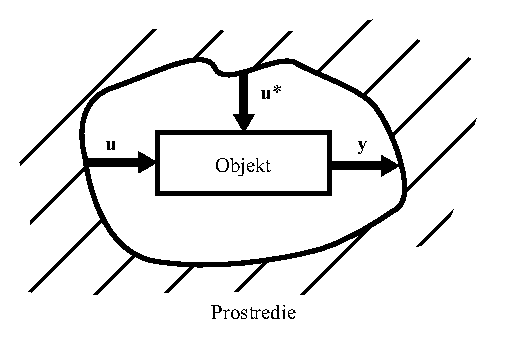
\includegraphics[width=80mm]{obr/OBRAZOK1_1.eps}
\caption{Stručný popis obrázku.}\label{OBRAZOK 1.1}
\end{figure}
%************ KONIEC **************
Nezabudnime, že popis obrázku je ukončený bodkou.

Na začiatku vety vypýšeme slovo Obrázok, kým všade inde používame skratku Obr.

\subsection{Formát obrázkov}

Pre ukladanie a zobrazenie obrázkov používame nasledovné súborové formáty:
\begin{itemize}
\item *.eps pre vektorovú grafiku (grafy, ilustrácie, priebehy)
\item *.png na screenshoty a
\item *.jpg na rasterovú grafiku (fotografie).
\end{itemize}

\subsection{Obrázky z Matlabu}

Z Matlabu exportujeme obrázky do formátu *.eps.

\section{Odvolávky na časti práce}
\label{hrusky}

Kapitolu, podkapitolu alebo podobné veci označíme príkazom "label", a nasledovne na nich odvoláme príkazom "ref". Napríklad v Kap. \ref{jablka} sme odvodili\ldots.
Na začiatku vety vypýšeme slovo Kapitola, kým všade inde používame skratku Kap. Podkapitoly a pod-podkapitoly v odvolávkach nerozlišujeme, na štruktúru dokumentu používame vždy Kap.

\section{Matematika}

Vzorce môžeme podľa potreby priamo písať do textu, napríklad: Číselná postupnosť - množina čísel $\vec{R} \{a_m, a_{m+1}, ...\}
= \{a_m\}_{m = n}^\infty$, respektíve to očíslovať a písať do samostatného riadku napríklad pomocou
  \begin{align}
  \label{mojarovnica}
    E_0 &= mc^2                              \\
    E &= \frac{mc^2}{\sqrt{1-\frac{v^2}{c^2}}}
  \end{align}
kde potom môžeme odvolávať na rovnicu pomocou Rov. \eqref{mojarovnica}. Pozor na to, že odkaz na čísla rovnice je zahrnutá v zátvorkách, to platí iba na rovnice, nie pre obrázky, tabuľky a štruktúru dokumentu. Namiesto príkazu align, môžeme používať aj eqnarray.

Na začiatku vety vypýšeme slovo Rovnica, kým všade inde používame skratku Rov.

\section{Programy, a užívateľské rozhrania}



\subsection{Programy}

Ak chceme písať názvy funkcií respektíve krátke časti počítačového kódu, môžeme na to používať príkaz \code{code}, napríklad \code{mojafunkcia()}.

Počítačový program môžeme jednoducho vložiť do textu pomocou
\lstset{language=exMatlab}
\begin{lstlisting}
N=1024;              % Pocet vzoriek
f1=1;                % Frekvencia harmonickeho signalu
FS=200;              % Frekvencia vzorkovania
n=0:N-1;             % Poradove cisla vzorky
x=sin(2*pi*f1*n/FS); % Generujeme signal, x(n)
[Rxx,Tau]=xcorr(x);  % Odhad autokorelacnej funkcie
\end{lstlisting}
Jazyk programu vieme určiť my, napríklad \code{Matlab} tu je rozšírený o extra príkazy.

\subsection{Užívateľské rozhrania}

Ak chceme označiť časti grafického rozhrania počítačového programu, cestu cez menu softvéru, názvy súborov atď, môžeme na to používať príkaz \code{gui}. Príkladom je \gui{File menu} alebo ikóna \gui{Môj počítač}.

\section{Tabuľky}


\begin{table}[htb]
\centering
\caption{Zoradenie metód na základe objemu apriórnych znalostí}
\begin{tabular}{ |l|c|c|c| }
  \hline
  \parbox[c]{3.5cm}{Metóda} & Kovariancia & \parbox[c]{3cm}{Hustota\\pravdepodobnosti}& Apriórna hustota\\ [0.2cm] \hline
  \parbox[c]{3.5cm}{Najmenšie štvorce} & Nie & Nie & Nie \\ [0.2cm] \hline
  \parbox[c]{3.5cm}{Najmenšie štvorce,\\Markov odhad}& Áno & Nie & Nie \\ [0.2cm]   \hline
  \parbox[c]{3.5cm}{Maximálna\\vierohodnosť}& Áno & Áno & Nie \\ [0.2cm] \hline
  \parbox[c]{3.5cm}{Bayesovské metódy} & Áno & Áno & Áno \\ [0.2cm] \hline
\end{tabular}
    \label{TABULKA_3_1}
\end{table}

Na tabuľky taktiež môžeme odvolávať pomocou Tab. \ref{TABULKA_3_1}. Tabuľky taktiež majú popis, dávame to nad tabuľkou.

Na začiatku vety vypíšeme slovo Tabuľka, kým všade inde používame skratku Tab.

\section{Fyzykálne jednotky}

Fyzikálne jednotky oddeľujeme medzerou od čísla a píšeme nezmeneným typom písma, t.j. nepoužívame šikmé písmo. Používame medzinárodne známe a akceptované jednotky a skratky jednotiek. Správne je teda 10 V, nesprávne je to 10V, 10 Volt, 10 \emph{V}.


\section{Bibliografické citácie}

Citovať môžeme nasledovne \cite{Eykhoff84}. Ak chceme citovať viacero autorov, tak môžeme to robiť naraz \cite{Fontes00,Eykhoff84}. Databazu citovaných dokumentov píšeme do súboru *.bib. Všetky typy dokumentov (kniha, článok etc.) má svoju vlastnú kategóriu. Autora publikácie môžeme aj napísať, napríklad že v práci Qin a Badgwell \cite{Qin99} dokázali že. Citácia je súčasťou vety, môžeme to kombinovať do vety \cite{Karny80} alebo dávať pred bodkou na koniec \cite{Far90}.

\section{Príklad}

Ak chceme uviesť inštrukčný príklad, potom na to máme prostredie
\begin{exmp}
Jožko má 5 melónov, vypočítajte hmotnosť Slnka.
\end{exmp}
kde príklad je ukončený znamienkom QED (štvorec).


\section{Záležitosti záverečnej práce}

\subsection{Obal}

Prvú stranu, takže obal a druhú (prázdnu stranu) nezviažeme do záverečnej práce, slúži to iba ako podklad na vyhotovenie obalu.

Na základe výnosu Ministerstva školstva Slovenskej republiky z 15. marca 2010 č. MŠSR-5/2010-071 ``o vzore obalu a titulného listu záverečnej, rigoróznej a habilitačnej práce a formáte výmeny údajov o záverečnej, rigoróznej a habilitačnej práci''  na obale záverečnej práce sa uvádzajú tieto informácie:
\begin{itemize}
\item  názov vysokej školy,
\item názov fakulty, ktorej je autor študentom, ak je zapísaný na štúdium študijného programu
uskutočňovaného na fakulte,
\item evidenčné číslo, ak bolo určené,
\item názov záverečnej práce, a ak sa použil, tak aj podnázov záverečnej práce,
\item meno, priezvisko, akademické tituly a vedecko-pedagogické tituly autora a
\item rok predloženia.
\end{itemize}

\subsection{Titulný list}

Na základe výnosu Ministerstva školstva Slovenskej republiky z 15. marca 2010 č. MŠSR-5/2010-071 ``o vzore obalu a titulného listu záverečnej, rigoróznej a habilitačnej práce a formáte výmeny údajov o záverečnej, rigoróznej a habilitačnej práci''  na titulnom liste záverečnej práce sa uvádzajú tieto informácie

\begin{itemize}
\item názov vysokej školy,
\item názov fakulty, ktorej je autor študentom, ak je zapísaný na štúdium študijného programu
uskutočňovaného na fakulte,
\item názov záverečnej práce, a ak sa použil, tak aj podnázov záverečnej práce,
\item označenie záverečnej práce: bakalárska práca, diplomová práca alebo dizertačná práca,
\item meno, priezvisko, akademické tituly a vedecko-pedagogické tituly autora,
\item názov študijného programu,
\item číslo a názov študijného odboru,
\item meno, priezvisko, akademické tituly a vedecko-pedagogické tituly školiteľa,
\item meno, priezvisko, akademické tituly a vedecko-pedagogické tituly konzultanta, ak bol pre
záverečnú prácu určený,
\item názov školiaceho pracoviska, ak pre záverečnú prácu bolo určené,
\item miesto a rok predloženia.
\end{itemize}


%Pisanie E, exponencia. nie e 

%\chapter{Ďalšie kapitoly}
\label{kap:3}
Každá kapitola začína na novej strane. Autor rieši zadanú problematiku. Na základe analýzy problému ponúka vlastné riešenia.

\section{Podkapitola}
\label{kap:1.1}

Podkapitoly záverečnej práce majú za úlohu členenie textu práce na dosiahnutie čo naj-väčšej prehľadnosti. Podkapitol môže byť viac, v ich názvoch sa používa desatinné číslovanie.

%[...]
\chapter{Záver}

Táto časť diplomovej práce je povinná. Autor práce uvedie zhodnotenie riešenia, jeho výhody resp. nevýhody, použitie výsledkov, ďalšie možnosti a podobne.  Môže aj načrtnúť iný spôsob riešenia úloh, resp. uvedie, prečo postupoval uvedeným spôsobom.


%%%%%%% Koniec %%%%%%%%
\bibliographystyle{abbrv}
\addcontentsline{toc}{chapter}{Literat\'{u}ra}
\bibliography{bibliog}
\end{document}
